\documentclass[12pt]{article}
\usepackage[margin=1in]{geometry}
\usepackage{longtable}
\usepackage{hyperref}
\usepackage{titlesec}
\usepackage{fancyhdr}
\usepackage{titling}
\usepackage{lmodern}
\usepackage{setspace}
\usepackage{graphicx}

\pagestyle{fancy}
\fancyhf{}
\rhead{Want2Remember SDD}
\lhead{Kevin Bayona-Galindo \\ Nikolazi Tartinsky}
\cfoot{\thepage}

\titleformat{\section}[block]{\normalfont\Large\bfseries}{\thesection}{1em}{}

\begin{document}

% Centered standalone title page
\begin{titlepage}
    \newcommand{\HRule}{\rule{\linewidth}{0.5mm}} 
    \vspace*{\fill}
    \begin{center}
        \HRule \\[0.5cm]
        {\Huge \bfseries Software Design Document \\[0.4cm]}
        \HRule \\[1.5cm]
        {\LARGE \textbf{Want2Remember Project}}\\[0.5cm]
        {\Large Final Documentation – May 6, 2025}\\[2cm]
        {\Large Kevin Bayona-Galindo \& Nikolazi Tartinsky}\\[0.5cm]
        {\large \today}
    \end{center}
    \vspace*{\fill}
\end{titlepage}

\tableofcontents
\newpage

\section*{Version History}
\begin{longtable}{|p{3cm}|p{3cm}|p{6cm}|p{4cm}|}
\hline
\textbf{Version} & \textbf{Date} & \textbf{Description} & \textbf{Authors} \\
\hline
v1.0 & 04/15/2025 & Initial requirement draft & Kevin \& Niko \\
\hline
v2.0 & 04/22/2025 & Added persistence and validation logic & Kevin \& Niko \\
\hline
v3.0 & 04/29/2025 & Included delete features and UI polish & Kevin \& Niko \\
\hline
v4.0 & 05/05/2025 & Finalized functional requirements and added test planning & Kevin \& Niko \\
\hline
\end{longtable}

\section{Introduction}
Want2Remember is a lightweight web application that enables users to create, view, and delete personal memory entries. It is built entirely using front-end technologies (HTML, CSS, JavaScript) and leverages `localStorage` to persist user data. This SDD outlines the system architecture, design decisions, component structure, and deployment approach of the application.

\section{System Architecture}
\begin{itemize}
  \item \textbf{Frontend:} HTML, CSS, JavaScript
  \item \textbf{Storage:} localStorage
  \item \textbf{Deployment:} Docker (NGINX)
  \item \textbf{Testing:} TestRail (Snapshots 2--4)
  \item \textbf{Project Tracking:} Jira (Sprint-based)
\end{itemize}

\subsection*{Workflow Diagram Description}
User accesses a form $\rightarrow$ submits memory $\rightarrow$ JavaScript stores it in \texttt{localStorage} $\rightarrow$ display updates dynamically $\rightarrow$ memory reloaded on refresh $\rightarrow$ user can delete memory $\rightarrow$ \texttt{localStorage} updates.

\section{Functional Requirements}
\begin{itemize}
  \item The system must allow users to add a memory entry that includes a title and note.
  \item The system must display all previously saved memory entries below the form.
  \item The system must allow users to delete individual memory entries.
  \item The application must persist user data using `localStorage` between sessions.
\end{itemize}

\section{Non-functional Requirements}
\begin{itemize}
  \item The app must function correctly in all modern browsers.
  \item The UI should be responsive and accessible.
  \item The app should not require internet access after initial loading.
  \item Page reloads must not erase saved data.
\end{itemize}

\section{External Interfaces}
\begin{itemize}
  \item HTML5 and CSS for UI
  \item JavaScript for logic and DOM manipulation
  \item Browser localStorage API for persistence
\end{itemize}

\section{Assumptions and Constraints}
\begin{itemize}
  \item No login or authentication is required.
  \item Data is stored on a per-browser basis.
  \item The app is primarily for desktop use, but responsive design supports mobile.
\end{itemize}

\section{User Interface Overview}
\begin{itemize}
  \item Clean, minimalist design with a form at the top and saved memories listed below.
  \item Confirmation message appears when a memory is saved.
  \item Each memory has a delete button for individual removal.
  \item Fully responsive layout for mobile and desktop use.
\end{itemize}

\section{Deployment Notes}
\begin{itemize}
  \item The application can be deployed using Docker with NGINX to serve static files.
  \item Developers can also run the app locally by opening `index.html` in a modern browser.
  \item A local development server such as Live Server can be used for real-time testing.
\end{itemize}

\section{References}
\begin{itemize}
  \item \url{https://developer.mozilla.org/en-US/docs/Web/API/Window/localStorage}
  \item \url{https://hub.docker.com/_/nginx}
  \item \url{https://www.docker.com/products/docker-desktop}
  \item \url{https://overleaf.com}
  \item \url{https://www.atlassian.com/software/jira}
  \item \url{https://github.com/kbthepioneer/Want2Remember-Final-Project}
\end{itemize}

\section{Workflow Diagram Image / System Architecture Image}

\begin{figure}[h!]
\centering
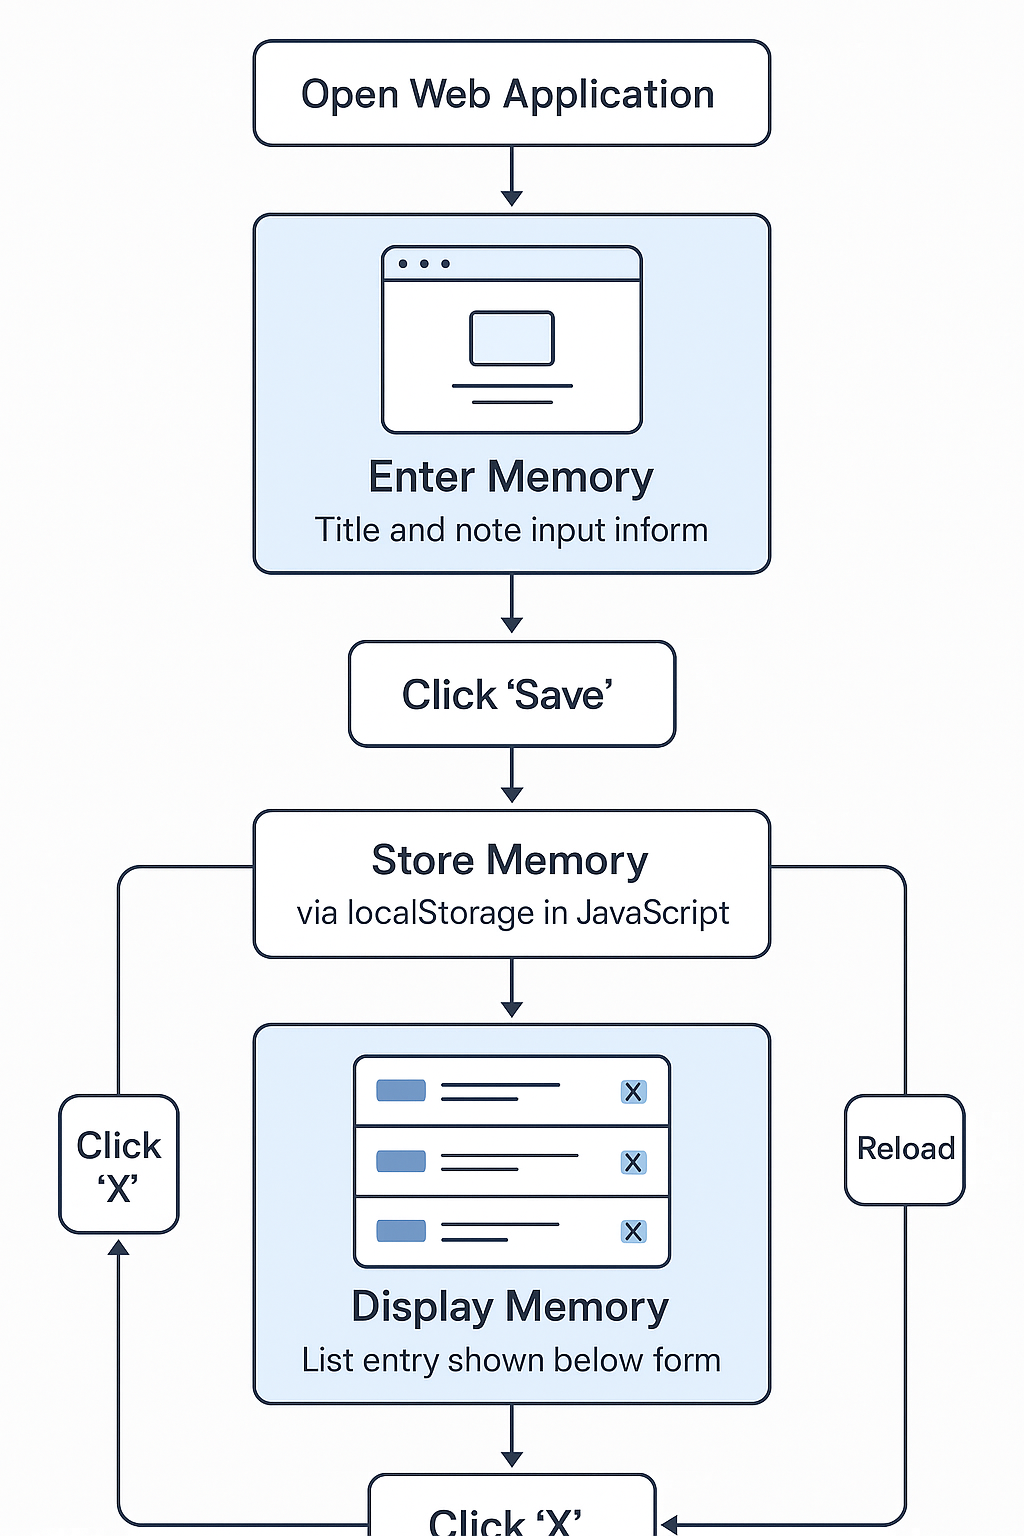
\includegraphics[width=0.8\textwidth]{workflow_diagram_FINAL.png}
\caption{Final Workflow Diagram}
\end{figure}

\begin{figure}[h!]
\centering
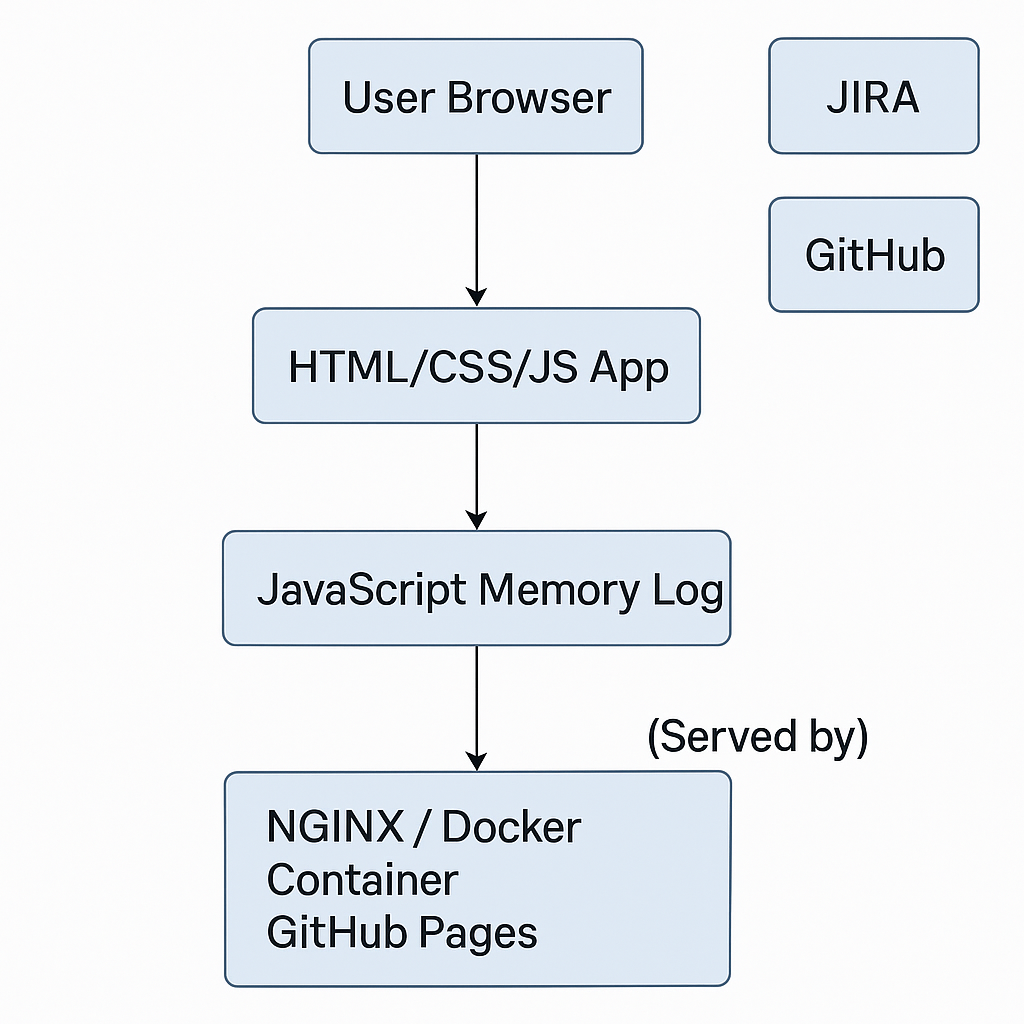
\includegraphics[width=0.8\textwidth]{system_architecture_FINAL.png}
\caption{System Architecture Diagram}
\end{figure}

\end{document}
